\documentclass[conference]{IEEEtran}
\IEEEoverridecommandlockouts
% The preceding line is only needed to identify funding in the first footnote. If that is unneeded, please comment it out.
\usepackage{cite}
\usepackage{amsmath,amssymb,amsfonts}
\usepackage{algorithmic}
\usepackage[dvipdfmx]{graphicx}
\usepackage{textcomp}
\usepackage{xcolor}
%\usepackage[dvipdfmx]{}
\setlength{\columnsep}{0.22 in}
\def\BibTeX{{\rm B\kern-.05em{\sc i\kern-.025em b}\kern-.08em
    T\kern-.1667em\lower.7ex\hbox{E}\kern-.125emX}}
%target AP
\newcommand{\SSID}{\rm SSID_{connect}}
\newcommand{\tarAP}{\rm AP_{connect}}
\newcommand{\tarMAC}{m_{connect}}
%user device
\newcommand{\userMAC}{m_{user}}
%input AP
\newcommand{\inputAP}{\rm AP_{owner}}
\newcommand{\inputMAC}{m_{input}}
%MAC address in sbxt
\newcommand{\stba}{m_{a}}
\newcommand{\stbA}{m_{A}}
\newcommand{\stbb}{m_{b}}
\newcommand{\stbB}{m_{B}}
\begin{document}

\title{Rogue Access Point Detection by Using ARP Failure under the MAC Address Duplication\\
\thanks{identify applicable funding agency here. If none, delete this.}
}

\author{\IEEEauthorblockN{Kosuke Igarashi, Hiroya Kato and Iwao Sasase}
\IEEEauthorblockA{\textit{Dept. of Information and Computer Science} \\
\textit {Keio University}\\
3-14-1 Hiyoshi, Kohoku, Yokohama, Kanagawa 223-8522, Japan, \\
Email: igarashi@sasase.ics.ac.keio.jp}

}
\maketitle
\begin{abstract}
Detecting a Rouge Access Point (RAP) in Wi-Fi network is imperative.
The previous scheme is user side detection focusing on two channels used by a RAP.
That scheme can detect a RAP in a stable traffic environment by revealing the channel used with a LAP with intentional interference.
However, the detection performance is degraded in the real environment where traffic is more unstable because it affects the channel interference.
Thus, it is necessary to design the scheme which is independent of such factors.
In this paper, we propose RAP detection by using Address Resolution Protocol (ARP) failure under the Media Access Control (MAC) address duplication.
Our main idea is that there exists a RAP and a Legitimate AP (LAP) on the same path under the attack.
This is because the RAP must be established between a user device and a LAP under the attack.
On the basis of this idea, the proposed scheme reveals that the AP with which a user device connects is a RAP by discovering the MAC address of a LAP on the same path.
In order to find the MAC address, we leverage the phenomenon that a user device cannot receive ARP reply packets in the situation where its MAC address and that of a AP are duplicated on the same path.
By doing this, the presence of a LAP is revealed, which can judge that the connected AP is a RAP.
In our evaluation, the proposed scheme achieves accuracy of 96.5\% even in unstable traffic environment.
True positive rate and false positive rate are 31.0\% higher and 9.0\% lower than the previous scheme.
Furthermore, the proposed scheme can detect RAPs accurately in a real environment where the previous scheme cannot.
\end{abstract}

\begin{IEEEkeywords}
Evil Twin Attack, Rogue Access Point, Address Resolution Protocol
\end{IEEEkeywords}

\section{INTRODUCTION}
With the rapid development of wireless communication techniques, Wi-Fi is deployed as the most commonly used Internet access technology and keeps spreading all over the world\cite{bg-evi}.
It is located in everywhere of our daily life, such as shopping malls, restaurants, public transit systems and so on.
While the free access to Wi-Fi network attracts a large number of users, it also allows adversaries to launch attacks to the users just by setting up a Rogue AP (RAP) on their laptop in the network, which is called ``Evil Twin Attack (ETA) ''\cite{laptop-evi}.
The RAP clones the Service Set IDentifier (SSID) and even Media Access Control (MAC) address of a Legitimate AP (LAP) provided by a public facility, which is the reason why it is called ETA.
In particular, cloning SSID enables adversaries to make user devices connect with a RAP because wireless devices connect automatically to an AP which has the strongest Received Signal Strength Indication (RSSI) among all APs with same SSID.
In the ETA, a RAP is established between a user device and the Internet as Man-In-The-Middle (MITM) attacks \cite{spoof-evi}.
Thus, adversaries can eavesdrop on the exchange of sensitive information such as identity credentials, passwords, and bank accounts by observing relayed packets through their laptop between a user device and a LAP.
In addition, adversaries can also carry out an active attack by leading a user to phishing websites or infecting a user device with malicious softwares\cite{research}.
By exploiting the characteristic that users freely connect free Wi-Fi network,  an adversary can succed in the attacks without being noticed by a user.
Thus, the detection of the RAPs is urgent demand.

The attack model is divided into two models based on how a RAP provides the Internet service to user device.
The one is a model where a RAP uses mobile communication, and it can be detected easily with Internet Services Provider (ISP) names or Global IP addresses\cite{rtt}.
Thus, we focus on the other model where a RAP uses same gateway with LAPs in the network by connecting with one of them since it cannot be easily detected by existing schemes.

Exisiting RAP detection schemes supposing this attack model are divided into network administrator side detections and user side detections.
The network administrator side detections mainly use whitelist-based mechanisms based on physical features of APs\cite{prapd}\cite{clockskew}.
However, those solutions are inapplicable to Wi-Fi hotspots since they make netowork addministrators set additional devices in their infrastructures.
On the other hand, the user side detections focus on communication features.
In particular, most of the exisiting schemes utilize network latency, such as Round-Trip Time (RTT) or Inter-packet Arrival Time \cite{rtt}\cite{iat}.
However, since such delay is caused by the software-based RAP on a laptop, latency based schemes can be easily evaded by using a hardware-based RAP.
Thus, in order to cope with both software-based RAPs and hardware-based ones, the user side detection scheme which focuses on two communication channels used by a RAP has been proposed \cite{previous}.
That scheme can detect the RAP by finding out these two channels on the basis of the decline in the throughput.
That scheme is the most useful detection since it can deal with a hardware-based RAP which does not cause delay.
Hence, we focus on that scheme \cite{previous} as the previous scheme.
Although the previous scheme is successful in the experimental environment, its detection performance is degraded by ubstable traffic in a real environment.
Therefore, it is necessary to realize the user side detection which is independent of the network traffic.

In order to realize the user side detection which is independent of a network environment, in this paper, we propose RAP detection by using Address Resolution Protocol (ARP) failure under the MAC address duplication.
The main idea of our scheme is that there exist two APs, namely the RAP and a LAP, on the same path from a user device to a gateway.
Therefore, in an attack scenario, besides the connected RAP, a LAP exists inevitably on the other side of the RAP because of the MITM attack.
On the basis of this idea, the proposed scheme reveals the connected AP as the RAP by finding MAC address of such a LAP from obtainable beacon frames by a user device \cite{beacon}.
In order to find the MAC address, we leverage the phenomenon that a user device cannot receive ARP reply packets from a gateway in the situation where its MAC address and that of a AP are duplicated on the same path.
The proposed scheme intentionally creates such situation by setting the MAC address of a user device to the one of a LAP on the same path.
By doing this, the proposed scheme can reveal the connected AP as a RAP regardless of network environment.
The contributions of our scheme are as follows:
\begin{enumerate}
    \renewcommand{\labelenumi}{\arabic{enumi}).}
    \item To the best of our knowledge, the proposed scheme is the first one which is independent of features of a RAP. By focusing only on the characteristic of attack and a MAC address of a LAP, the proposed scheme does not allow an adversary to avoid detection by manipulating features of the RAP.
    \item The proposed scheme achieves accurate detection performance without any error even in a real environment. It can guarantee beneficial effects on every available hotspot.
\end{enumerate}
The rest of this paper is constructed as follows: Related works are described in Section \ref{sec:2}.
The attack model, previous scheme and its shortcoming are intriduced in Section \ref{sec:3}.
The proposed scheme is explained in Section \ref{sec:4}.
Various evaluation results are shown in Section \ref{sec:5}.
Finally, the conclusions of this paper are presented in Section \ref{sec:6}.

\section{RELATED WORKS}\label{sec:2}
RAP detection methods are mainly classified into two categories: network administrator side detections and user side detections.
Network administrator side detections \cite{prapd}\cite{clockskew} focus on the physical features such as RSSI and clock skew which cannot be spoofed by an adversary.
A RAP can be detected by comparing with the physical features of it with those in the predefined whitelist with equipments such as traffic sensors in each Wi-Fi network.

Wu et al. \cite{prapd} pay attention to the RSSI which is hard to be forged arbitrarily and highly correlated to the transmitter's location and power.
For each LAP in a network, RSSI, which is measured by additional costly devices, is registered as the information in a whitelist beforehand.
By using RSSI, even if the MAC address of an AP is identical to that in the whitelist, that scheme can disclose that it is a RAP with spoofed MAC address set by an adversary at different location.
However, that scheme is hard to detect RAP which is located near the LAP because RSSI is not as exact as it can indicate a small difference of the nearby location.
Although RSSI is useful as a supplementary feature, using only RSSI is insufficient to detect a RAP with high accuracy.

In order to detect in more detail, Lanze et al. \cite{clockskew} focus on clock skew as a device fingerprinting based purely on physical properties.
Clock skew is the time gap of clock signals caused by the crystal oscillator, which is one of the components equipped in each AP.
Since the clock skew is a precise feature which is unique to each AP, that scheme can be useful.
However, that scheme is inapplicable to Wi-Fi hotspots because it requires additional costly sensors for obsering the feature.
Administrators are required to set up additional devices in their infrastructures.
Thus, the detection schemes that require no equipment of additional devices by a network administrator are desired.

Meanwhile, user side detections \cite{rtt}\cite{previous} do not need to introduce additional devices to a Wi-Fi hotspot.
They focus on differences in the transmission characteristics caused by the extra hop to a RAP on the path between a LAP and a user device.
Compared with legitimate networks, extra hop results in several measurable changes in transmission characteristics such as RTT and channel used between a user device and DNS server.

Mustafa et al. \cite{rtt} differentiate RAPs from LAPs by measuring the RTT between the user device and the DNS server through different target APs (RAPs or LAPs).
Because there exists the extra hop caused by the RAP on the path, RTT is longer in comparison to the case where a user directly connects to the LAP.
Although that scheme is useful only for the case where the adversary sets RAP up on the laptop, Jang et al. \cite{previous} reveal the fact that the computational power of the software bridging mainly accounts for the packet delay.
Thus, the adversary can evade the packet delay based detection by utilizing hardware-based RAPs having little bridging delay unlike software-based RAPs.

In order to detect both types of RAPs, namely, software-based and hardware-based ones, Jang et al. focus on two communication channels utilized by a RAP between a user device and LAP\cite{previous}.
Whereas a RAP intervenes between a user device and a LAP, two distinct channels are used to reduce communication delay caused by channel interference each other.
For example, it is assumed that channel 1 is used as the channel between a user device and a RAP, and channel 6 is that between the RAP and a LAP.
That scheme detects RAP by finding out the presence of these two channels with the throughput of the transmission from the user device to the DNS server.
That scheme is the most robust user side detection which is independent of the performance of the RAP because it is the countermeasure against a reasonable attack model where hardware-based RAP is used.
Thus, we select the scheme \cite{previous} as the previous scheme.
In the next section, we elaborate the previous scheme.

\section{ATTACK MODEL AND PREVIOUS SCHEME}\label{sec:3}
\begin{figure}[t]
    \begin{center}
        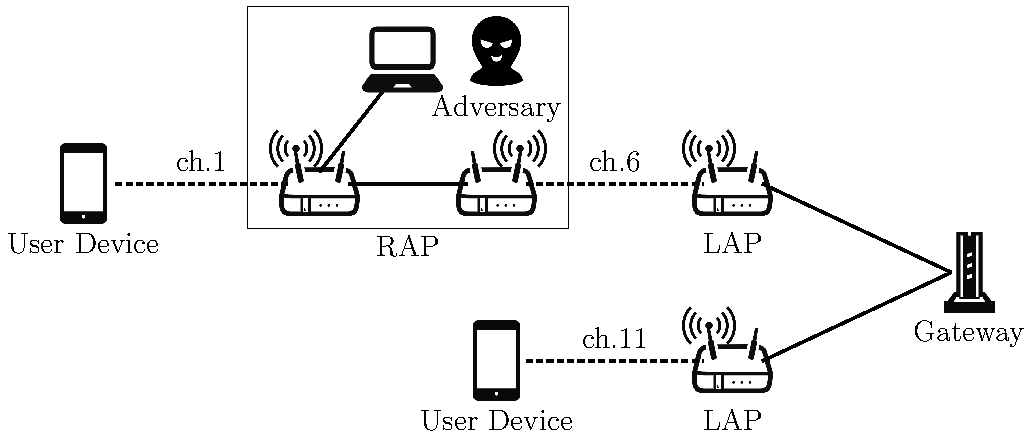
\includegraphics[scale=0.5]{attack-model/attack-model.pdf}
        \caption{The Attack Model}
        \label{fig:model}
    \end{center}
\vspace{-2zh}
\end{figure}
\subsection{Attack Model}
In an ETA, the adversary sets up a RAP which uses a SSID of a LAP in the targeted Wi-Fi network.
Besides, the MAC address of the RAP is cloned from one of the LAPs in the network\cite{spoof-evi}.
As a result, although a user device receives SSID broadcast from the RAP and LAPs, it cannot differentiate between these APs.
Thus, since the user device simply connects with the AP that has a higher RSSI value, the RAP sends beacon frames with stronger signals.
\figurename~\ref{fig:model} shows the attack model.
We assume that a RAP relays packets between a LAP and a user device, which acts as a MITM attack to steal private information of a user.
By avoiding using mobile Internet access, e.g., 3G/4G, the adversary can evade simple detections with Internet Services Provider (ISP) names or Global IP addresses \cite{rtt}.
In addition to that, we assume that the adversary exploits hardware-based APs in order not to cause a computational delay \cite{previous}.
In order to use distinct channels on the both sides, a RAP is composed of two routers which are interconnected with a LAN cable.
One of these routers is connected to a LAP in station mode and the other disguise user device as a LAP in service mode.
Because a high-end router which can relay packets with distinct channels appears nowadays, it can replace a RAP in our model.

\subsection{Previous Scheme}
\subsubsection{Overview of the Previous Scheme}
The main idea of the previous scheme \cite{previous} is that the adversary needs to use two distinct communication channels on the path from a user device to the LAP to avoid channel interference each other.
The one is the channel for the path between a LAP and a RAP, and the other is that for the path between a RAP and the user device.
Thus, from the perspective of the user device, there exists another channel on the route that is different from the channel with the connected AP.
The extra channel cannot be observed directly from the user device.
The previous scheme detects the RAP by finding out these two channels on the basis of the decline in the throughput.
In order to decrease the throughput, the previous scheme saturates the channel used between a LAP and the RAP by intentionally interfering a channel with an additional equipment in a user device.
For example, when a user device is using channel 1 with the connected AP which cannot be judged to be legitimacy, the equipment in a user device transmits a large number of packets to all the channel except channel 1 to saturate traffic on the path.
If there exists the other channel on the route, the decline in the throughput can be observed by the user device, and the presence of RAP is revealed.

\subsubsection{Shortcoming of the Previous Scheme}\label{sec:shortcoming}
\begin{figure}[t]
    \begin{center}
        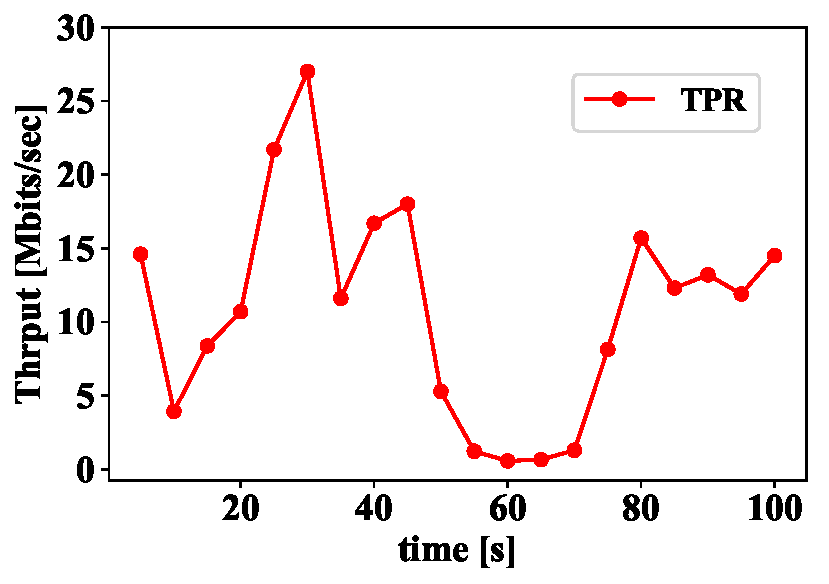
\includegraphics[scale=0.3]{figure/Thrput.pdf}
        \caption{Throughput in a Cafe}
        \label{thrput}
    \end{center}
    \vspace{-2zh}
\end{figure}
Although the previous scheme is successful in the detection for a hardware-based RAP in the experimental environment, it cannot detect the RAP accurately in the real world.
This is because throughput is considerably dependent on various factors of the network environment such as mobility of the traffic, collisions, network topology changes, and unintentional interference.
\figurename~\ref{thrput} shows the graph regarding the change of throughput in a cafe on a weekday.
As shown in \figurename~\ref{thrput}, since the traffic in real environment is unsteady in fact, the previous scheme is subject to environmental changes, which can lead to degrade the detection performance.
Thus, the requirement that we must satisfy is to leverage factors which are independent of the network environment for the detection.

\section{PROPOSED SCHEME}\label{sec:4}
In order to meet the requirements mentioned in Section \ref{sec:shortcoming}, in this paper, we propose RAP detection by using ARP failure under the MAC address duplication.
In the following subsections, we explain the idea of the proposed scheme and the algorithm in detail.

\subsection{Idea}
The main idea of the proposed scheme is that there exist two APs, namely, the RAP and a LAP, on the same path from a user device to a gateway.
In general, a LAP is the only device which exists on the path.
Therefore, in this case, the LAP is identical to the AP directly connected with a user device.
In an attack scenario, besides the connected AP, a LAP exists inevitably on the other side of the AP.
Therefore, a connected AP can be revealed as the RAP when the presence of a LAP is detected on the same path.

On the basis of this idea, the proposed scheme reveals a LAP is on the other side of the connected AP by finding out the MAC address of the LAP.
In order to discover the MAC address of a LAP on the same path, we leverage the phenomenon that a user device cannot receive ARP reply packets in the situation where there exist duplicate MAC addresses on the same path.
The proposed scheme intentionally creates such situation by setting the MAC address of a user device to the MAC addresses obtained from beacon frames of APs in the communication range of a user device.
Note that the MAC address of the AP with which a user device connects is excluded from targets for setting MAC addresses.
If the MAC address of a user device is set to that of a LAP on the same path, the LAP receives ARP reply packets whose original destination is the user device before the user device receives them.
Thus, since the user device cannot receive ARP reply packets, it continues to resend ARP requests, which results in disabling internet connectivity.
By observing the continuance of resending ARP request packets within a definite period of time without ARP reply packets, the proposed scheme can reveal that there exists the RAP and a LAP on the path, which detects the attack. %reply $B$,Mh$k$^$GAw$jB3$1$^$9(B

When a user device connects with the RAP, there exists a MAC address of a LAP in the communication range of a user device.
This is because the RAP is located relatively near a LAP to avoid communication delay.
Hence, we can inevitably obtain the MAC address of a LAP in the case where there exists the RAP in a network.
In the real situation, it is possible that there exist several LAPs in a communication range of a user device.
Thus, we collect the only MAC addresses of APs which have the identical SSID to that of APs in the network.
This is because a RAP must utilize an SSID of a LAP for pretending to be a LAP.
A user device can receive ARP reply packets even if its MAC address is set to that of each LAP on distinct paths.
This is because the MAC addresses can be duplicated except those on the same path.

Since the proposed scheme is independent of the real network environment, it is useful for overcoming the shortcoming of the previous scheme.
In addition to that, the proposed scheme is not affected by a spoofed MAC address because it focuses on the only legitimate MAC address never spoofed.

\subsection{Algorithm} \label{sec:alg}
\begin{figure}[t]
    \begin{center}
        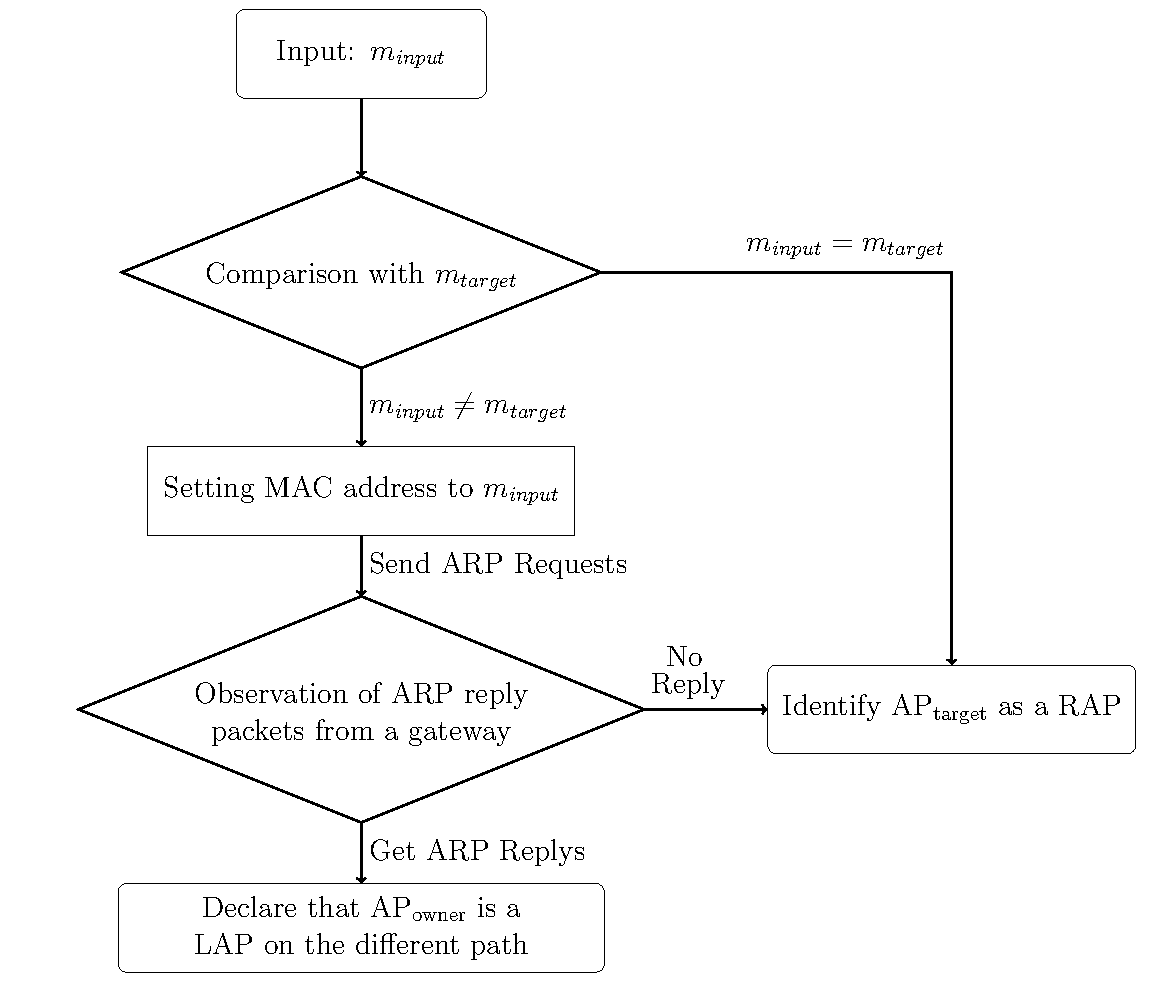
\includegraphics[scale=0.45]{flowchart/flowchart.pdf}
        \caption{The Flowchart of the Proposed Scheme}
        \label{fig:flowchart}
    \end{center}
\vspace{-2zh}
\end{figure}
In this subsection, the algorithm for the detection based on searching the MAC address of a LAP on the same path is explained.
The proposed algorithm mainly consists of 1) MAC address collection and 2) ARP reply based detection.

\subsubsection{MAC Address Collection}
Let $\tarAP$, $\SSID$ and $\tarMAC$ denote a AP which connects with a user's device, its SSID and its MAC address, respectively.
The set of MAC addresses of APs whose SSIDs are identical to $\SSID$  is created through beacon frames of them.
Let the set is denoted by $M_{all}=\{m_{input}|0\le input \le n_{all}  \}$, where $n_{all}$ is the number of collected MAC addresses.

\subsubsection{ARP Reply based Detection}
\figurename~\ref{fig:flowchart} shows the flowchart of this phase.
As shown in \figurename~\ref{fig:flowchart}, this phase consists of three procedures which are a) Comparison with $\tarMAC$, b)Setting MAC address, and c) Observation of ARP reply from the gateway to the user device.
These procedures are repeatedly conducted for every $m_{input}$ in $M_{all}$ unless the RAP is detected.

In the first phase, $\inputMAC$ and $\tarMAC$ are compared.
If they are the same MAC address, it easily judges that $\tarMAC$ is the cloned address.
In this case, since $\tarAP$ is detected as the RAP, the detection is finished.
However, in the case where the RAP clones a MAC address of a LAP beyond the communication range of a user's device or it does not clone, the accordance of MAC addresses cannot be detected only by this MAC address checking.
Thus, the detection process proceeds to the second phase.

In the second phase, the MAC address of a user device is set to $\inputMAC$.
After the MAC address is set to $\inputMAC$, the connection between the user device and $\tarAP$ is once lost since the gateway become unable to use the original MAC address as a destination for the packets.
Thus, the user device sends ARP request in order to reconnect with it through the $\tarAP$ automatically because of the stronger RSSI than any other APs.

Finally, in the third procedure, the ARP reply packets whose destination is set as $\inputMAC$ are observed to investigate whether the AP with $\inputMAC$, is on the same path with the user's device.
If the packets do not reach the user's device, the $\tarAP$ can be revealed as the RAP which exists between the user device and the LAP with $\inputMAC$, and the detection phase is finished.
Otherwise, the $\tarAP$ is judged that it is on the distinct path from the AP with $\inputMAC$.
In this case, the same procedures in the flowchart are repeatedly conducted for another $\inputMAC$ in $M_{A_{all}}$ until the RAP is detected.
If the detection phase is carried out for all $\inputMAC$ without the detection of RAP, the $\tarAP$ is declared as a LAP. 
\begin{figure*}[ht]
    \begin{minipage}{0.33\hsize}
        \begin{center}
            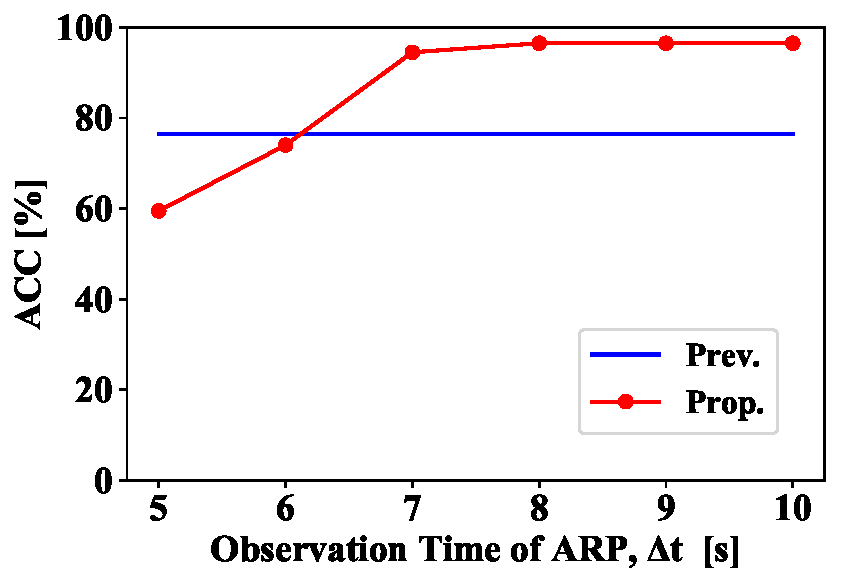
\includegraphics[scale=0.35]{figure/ACC.pdf}
        \end{center}
        \caption{The Avg. ACC of the Prop. and Prev.}
        \label{fig:acc}
    \end{minipage}
        \begin{minipage}{0.33\hsize}
        \begin{center}
            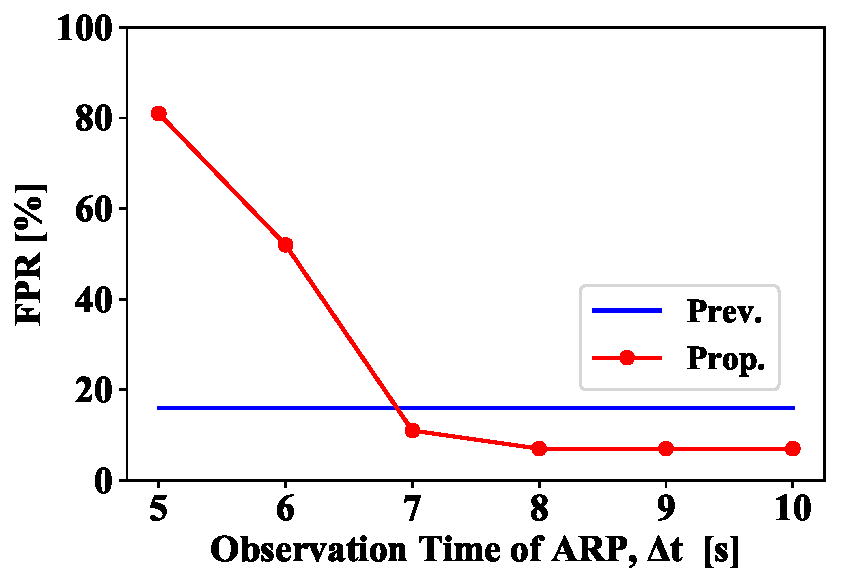
\includegraphics[scale=0.35]{figure/FPR.pdf}
        \end{center}
        \caption{The Avg. FPR of the Prop. and Prev.}
        \label{fig:fpr}
    \end{minipage}
    \begin{minipage}{0.33\hsize}
        \begin{center}
            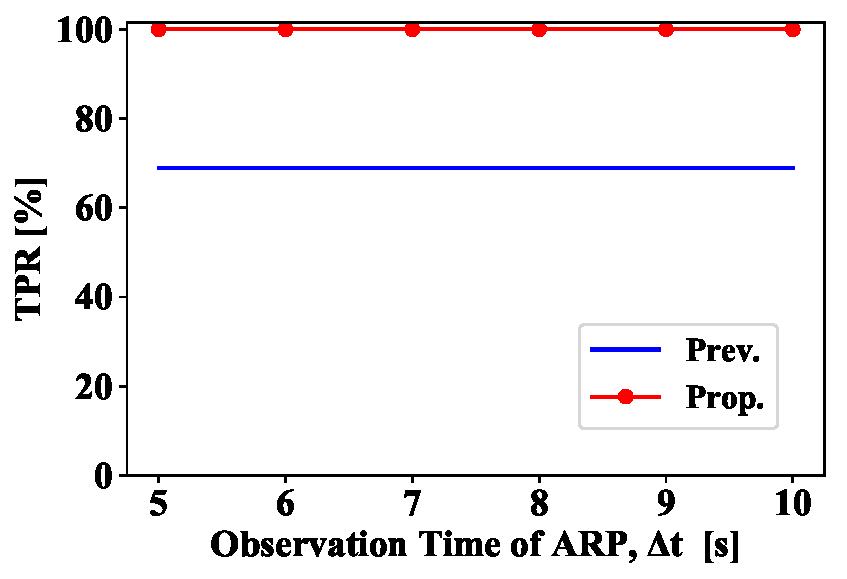
\includegraphics[scale=0.35]{figure/TPR.pdf}
        \end{center}
        \caption{The Avg. TPR of the Prop. and Prev.}
        \label{fig:tpr}
    \end{minipage}
\vspace{-1zh}
\end{figure*}
\section{EVALUATION}\label{sec:5}
In order to demonstrate the effectiveness of the proposed scheme, we compare it with the previous scheme \cite{previous} which interferes the channel between a LAP and a RAP.

The metrics of the evaluation are ACCuracy (ACC), True Positive Rate (TPR), and False Positive Rate (FPR) defined as
\begin{gather}
    \mathrm{ACC} = \frac{\mathrm{TP} + \mathrm{TN}}{\mathrm{TP} + \mathrm{TN} + \mathrm{FP} + \mathrm{FN}}, \\
    \mathrm{TPR} = \frac{\mathrm{TP}}{\mathrm{TP} + \mathrm{FN}}, \\
    \mathrm{FPR} = \frac{\mathrm{FP}}{\mathrm{FP} + \mathrm{TN}},
\end{gather}
where TP, TN, FP, and FN denote the number of True Positive (RAPs are regarded as RAPs), True Negative (LAPs are regarded as LAPs), False Positive (LAPs are regarded as RAPs), and False Negative (RAPs are regarded as LAPs), respectively.
We evaluate the proposed scheme with these metrics in two scenarios which are the case of attack where a user device connects with a RAP and that of non-attack where a user device connects with a LAP.

\subsection{Experimental Setup}
\subsubsection{Detector}
We implemented the detectors in a laptop, which is a MacBook Pro with an Intel Core i5 CPU.
We observe ARP packets with T-shark, which is a tool for capturing packets\cite{wire}.
Besides, in order to reproduce the detection model in the previous scheme \cite{previous}, we use a TP-Link Archer C6 as an interference device.

\subsubsection{LAP and RAP}
TP-Link Archer C6 is also used to setup the LAP.
As regards the RAP, in order to use distinct channels on both sides as the model in the previous scheme, it is composed of two APs (TP-Link Archer C6 and TP-Link Archer C50).
These two APs, where one is in the station mode ($\rm AP_{sm}$) and the other is in AP mode ($\rm AP_{am}$), are interconnected using a LAN cable.
The $\rm AP_{sm}$ is responsible for repeating packets to and from the LAP, and the $\rm AP_{am}$ has a spoofed SSID and MAC address.
All devices are operated in the IEEE 802.11n mode with MIMO.
We arrange a LAP, a RAP, and a user device at equal intervals which are 5 feet.

\subsubsection{Traffic Scenario}
In order to demonstrate the robustness against unstable traffic in real environment, we intentionally generate random traffic to the LAP at random time.

\subsubsection{Time of Detection}
The experiments are conducted for each case, namely attack scenario and non attack scenario 100 times.
The average time required per detection is represented as $T$.
It is affected by the observation time of ARP procedure per a AP, which is represented as $\Delta t$ , and also the number of LAPs before a RAP is detected in an attack scenario.
We conducted each evaluation by changing $\Delta t$ from 5 seconds to 10 seconds at every second.

\subsection{Evaluation of the Proposed Scheme}
In order to show the effectiveness of the proposed scheme (Prop.), we compare it with the previous scheme \cite{previous} (Prev.).
\figurename~\ref{fig:acc} shows the results of the average ACC over the 100 experiments in each scheme.
As shown in \figurename~\ref{fig:acc}, Prev. cannot accurately detect the attack in random traffic scenario, and the ACC is about 69\%.
However the ACC of the Prop. is lower than that of the Prev. when each ARP observation time is not greater than 6s.
The ACC is getting higher as the observation time increases.
In particular, in the case where the time is longer than 7s, ACC is improved up to 96.5\% in the Prop..
\figurename~\ref{fig:fpr} shows the FPR of each scheme.
As shown in \figurename~\ref{fig:fpr}, the longer each observation time is, the lower FPR is in the Prop..
It decreases up to 74\% in the case where $\Delta t$ is no less than 8 seconds compared with the case where $\Delta t$ is 5 seconds.
In additon, \figurename~\ref{fig:tpr} shows the TPR of each scheme.
As shown in \figurename~\ref{fig:tpr}, TPR of the Prop. is 100.0\% regardless of the observation time, which means it never pass a RAP over in an attack scenario. 

In order to reveal the reason of these results, we analyze the ARP packets in detail.
Through the packet analysis, we disclose the reason is that the time for finishing ARP procedure tends to be longer than 6s and it is not always fixed.
Thus, in the case of less than 7.0 seconds, several LAPs are detected as RAPs incorrectly since it is not enough for a user device to get ARP reply packets while a RAP is never overlooked. 
Given the fact, we conducted the further experiment to realize more precise detection by setting enough time to auquire ARP reply packets.
As a result, we conclude that the proposed scheme enables the detection without any error when the $\Delta t$ is set to 15 seconds.

\subsection{Evaluation in a Real Environment}
\begin{figure}[t]
    \begin{center}
        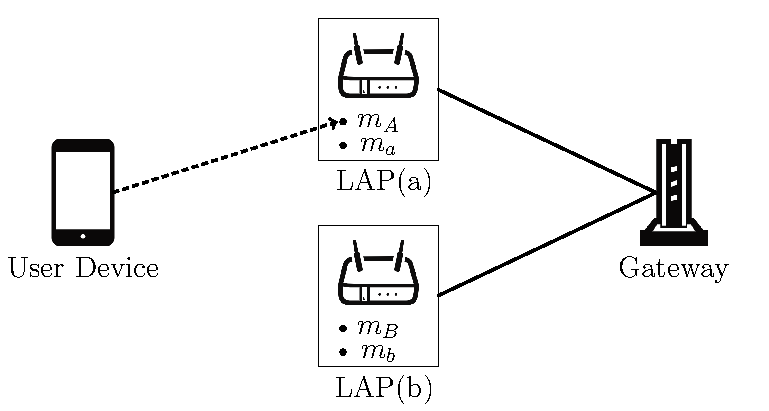
\includegraphics[scale=0.5]{starbucks/starbucks.pdf}
        \caption{The Network Model in the Cafe}
        \label{fig:sbx}
    \end{center}
    \vspace{-1zh}
\end{figure}
In order to demonstrate the robustness and the average time per detection time $T$ of the proposed scheme in a real environment, we conducted an experiment in a cafe and evaluate ACC and the total time required for the detection.
\figurename~\ref{fig:sbx} shows the Wi-Fi network model in the cafe.
As shown in \figurename~\ref{fig:sbx}, there exist two LAPs, which are LAP(a) and LAP(b), and the both have same SSID and two different MAC addersses for two frequency bands which can be used in IEEE 802.2n.
The MAC addresses of LAP(a) are represented as $\stbA$ and $\stba$ , and similarly, those of LAP(b) are represented as $\stbB$ and $\stbb$.
Through the evaluations, the user device is always connected to $\stbA$.
In non attack scenario, we use $\stbB$ and $\stbb$ as MAC address in the set of $M_{all}$ defined in Section \ref{sec:alg}.
In contrast, we construct the attack scenario experimentally by assuming $\stbA$ and $\stba$ as the MAC address of a RAP and that of a LAP which is on the same path with RAP since an acutual RAP cannot be installed in a real world.
In this case, the RAP is regarded as the high-end router which can relay packets with distinct channels.
In order to match the number of the MAC addesses which need to be input to the proposed scheme, we only use $\stba$ and $\stbb$ in the attack scenario.
Our experimental situation can be regarded as the same situation with the attack model shown in \ref{fig:model}.
The experiments are conducted 100 times in each situation around 2:00pm on a weekday at an cafe.
$\Delta t$ is set to 15 seconds enough to get ARP reply packets.
\begin{table}[t] 
    \begin{center}
        \caption{Evaluation Result in Real Environment}
        \label{tab:real}
        \begin{tabular}{c c} \hline
            ACC (\%) & Avg. Total Time (s) \\ \hline \hline
            100.0 & 32.1 \\ \hline
        \end{tabular}
    \end{center}
    \vspace{-2zh}
\end{table}

\tablename~\ref{tab:real} shows the results in the real environment.
The proposed scheme realizes 100\% accuracy even in a real environment if $\Delta t$ is enough.
At that time, $\rm T$ is 32.1 seconds.
It is much shorter than the time that the most of recent security softwares take to scan their disk.
Thus, it guarantees the device's safety for users without being annoyed.
Through this result, we conclude that the proposed scheme can accurately detect the attack with relatively short time in a real environment whose traffic is unstable.

However, as with other existing schemes, the proposed scheme assumes Wi-Fi network models where Legitimate Repeaters (LR) are not installed.
It may be usual to introduce a LR in network to relay traffic farther at the expense of transmission speed in a large area.
In this case, the proposed scheme cannot distinguish a RAP and LR since both of them relay packets between a user device and a LAP in the same way as MITM attack.
In order to detect the attack even in such Wi-Fi networks, we focus on their RSSI values as supplementary features because it can tell their general distance each other \cite{rssi}.
Since a LR has a function to relay packets from a LAP to devices which cannot connect with the LAP because of the long distance, it should be located far from a LAP in general.
In contrast, a RAP is basically introduced near a connecting LAP not to cause traffic delay due to their long distance.
Thus, we assume that an AP can be judged whether it is a LR or not on the basis of this idea.
In the future, we plan to devise the additional countermeasures and conduct some experiments so as to distinguish LR with RSSI value.

\section{conclusion}\label{sec:6}
In this paper, we have proposed RAP detection by using ARP failure under the MAC address duplication.
We collect MAC addresses from user side and set the MAC address of a user device to them.
By observing ARP packets in the situation, we can reveal the legitimacy of connected AP.
The detection performance of the proposed scheme is better than the previous scheme.
The results show it can detect a RAP without any error even in unstable traffic environment.
In addition, the experiment in a small cafe shows the availability in a real network.
In the future, we will conduct a large-scaled examination of the proposed scheme.
Furhermore, we will expand the scheme for the network where a legitimate repeater is arranged.

\section*{acknowledgment}
This work is partly supported by the Grant in Aid for Scientific Research (No.17K06440) from Japan Society for Promotion of Science (JSPS).


\bibliographystyle{IEEEtran}
\bibliography{IEEE_ref}
\vspace{12pt}
\end{document}
